\documentclass{article}
\usepackage[UTF8]{ctex}
\usepackage{amsfonts}
\usepackage{amsmath}
\usepackage{float}
\usepackage{graphicx}
\usepackage{url}

\newcommand{\Bezier}{B\'ezier}%Bézier

\usepackage{color}

% paragraph
\setlength{\parindent}{0pt}
\setlength\parskip{\baselineskip}
\renewcommand{\baselinestretch}{1.2}

\begin{document}
	
	% 标题
	\title{《计算机辅助几何设计》作业}
	\author{ID号: 048  \qquad  姓名: 郑涛}  %递交作业时填上ID号和姓名
	\date{2024年10月5日}
	\maketitle
	
	
	1. Prove: The arc length of a \Bezier curve is not greater than the perimeter
	of its control polygon.\\
	证明:
	
	\qquad设控制点为$P_0,P_1,\dots,P_n$生成的\Bezier曲线为:
	$$B(t)=\sum_{i=0}^{n}C_n^it^i(1-t)^{n-i}P_i$$
	\qquad一阶导数为:
	$$B'(t)=n\sum_{i=0}^{n-1}C_{n-1}^it^i(1-t)^{n-i-1}(P_{i+1}-P_i)$$
	\qquad运用范数的三角形不等式可以得到:
	$$||B'(t)||\leq n\sum_{i=0}^{n-1}C_{n-1}^it^i(1-t)^{n-i-1}\cdot||P_{i+1}-P_i||$$
	\qquad两边积分:
	$$\int_{0}^{1}||B'(t)||dt\leq n\sum_{i=0}^{n-1}C_{n-1}^i\int_{0}^{1}t^i(1-t)^{n-i-1}dt\cdot||P_{i+1}-P_i||$$
	\qquad其中,
	$$\int_{0}^{1}t^i(1-t)^{n-i-1}dt = \frac{i!(n-i-1)!}{n!}$$
	$$nC_{n-1}^i\int_{0}^{1}t^i(1-t)^{n-i-1}dt=n\cdot \frac{(n-1)!}{i!(n-i-1)!}\cdot\frac{i!(n-i-1)!}{n!}=1$$
	\qquad于是就有:
	$$\int_{0}^{1}||B'(t)||dt\leq\sum_{i=0}^{n-1}||P_{i+1}-P_i||$$
	\qquad右端即为控制点的折线长度。证毕
	
	
	2. Prove: A circular arc cannot be represented exactly by a Bézier curve.\\
	证明:
	
	\qquad我们熟知,圆弧的曲率为定值,只需证明贝塞尔曲线的曲率不为定值即可。
	
	\qquad设控制点为$P_0,P_1,\dots,P_n$生成的\Bezier曲线为:
	$$B(t)=\sum_{i=0}^{n}C_n^it^i(1-t)^{n-i}P_i$$
	\qquad一阶导数为:
	$$B'(t)=\sum_{i=0}^{n-1}C_n^i(n-i)t^i(1-t)^{n-i-1}(P_{i+1}-P_i)$$
	%\qquad一阶导数的最高次项系数为:
	%$$\sum_{i=0}^{n-1}C_n^i(n-i)(-1)^{n-i-1}(P_{i+1}-P_i)=n\sum_{i=0}^{n-1}C_{n-1}^i(-1)^{n-i-1}(P_{i+1}-P_i)$$
	\qquad二阶导数为:
	$$B''(t)=\sum_{i=0}^{n-2}C_n^i(n-i)(n-i-1)t^i(1-t)^{n-i-2}(P_{i+1}-2P_{i+1}+P_i)$$
	\qquad Bézier曲线的曲率为:
	$$K_B(t)=\frac{|B'(t)\times B''(t)|}{|B'(t)|^3}$$
	\qquad设Bézier曲线中$t$的最高次数为$r(2\leq r\leq n)$,则一阶导数的最高次数为$r-1$,二阶导最高次数为$r-2$,则分子中$t$的次数不超过$2r-3$,分母中t的次数为$3r-3\textgreater 2r-3$,因此$K_B(t)$不为常函数,这也就证明了Bézier曲线无法精确表示一段圆弧。
	
	3. Try to calculate the area of the region enclosed by a planar nth-degree
	\Bezier curve, its first and last control points, and the origin (as shown in
	the gray area in the figure below). Express the result using the coordinates
	of the control points.\\
	\begin{figure}[H]
		\centering
		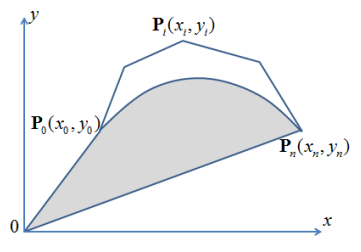
\includegraphics{a}
		\label{fig:a}
	\end{figure}
	证明:
	
	\qquad设控制点为$P_0,P_1,\dots,P_n$生成的\Bezier曲线为:
	$$B(t)=\sum_{i=0}^{n}C_n^it^i(1-t)^{n-i}P_i=(B_x(t),B_y(t))$$
	\qquad一阶导数为:
	$$B'(t)=\sum_{i=0}^{n-1}C_n^i(n-i)t^i(1-t)^{n-i-1}(P_{i+1}-P_i)=(B_x'(t),B_y'(t))$$
	\qquad Bézier曲线上关于参数$t$距离足够近的两点记为$P(B_x(t),B_y(t))$,\\$Q(B_x(t+\Delta t),B_y(t+\Delta t))$,该两点与原点形成了一个三角形微元$\Delta OQP$,其有向面积为:
	\begin{equation*}
		\begin{aligned}
			A_{\Delta OQP}=&\frac{1}{2}[B_x(t+\Delta t)B_y(t)-B_x(t)B_y(t+\Delta t)]\\
			=&\frac{1}{2}[B_x(t)+\Delta tB_x'(t)]B_y(t)-B_x(t)[B_y(t)+\Delta tB_y'(t)]\\
			=&\frac{1}{2}\cdot\Delta t\cdot [B_x'(t)\cdot B_y(t)-B_x(t)\cdot B_y'(t)]
		\end{aligned}
	\end{equation*}
	\qquad因此题目所要求的总面积为:
	\begin{equation}
		\label{A}
		\begin{aligned}
			A=\frac{1}{2}\int_{0}^{1}[B_x'(t)\cdot B_y(t)-B_x(t)\cdot B_y'(t)]dt
		\end{aligned}
	\end{equation}
	\qquad先求$\int_{0}^{1}B_x'(t)\cdot B_y(t)dt$,另一部分只需交换$x,y$即可。
	\begin{equation*}
		\begin{aligned}
			\int_{0}^{1}B_x'(t)\cdot B_y(t)dt=&\int_{0}^{1}[\sum_{i=0}^{n-1}C_n^i(n-i)t^i(1-t)^{n-i-1}(P_{i+1}-P_i)_x][\sum_{j=0}^{n}C_n^jt^j(1-t)^{n-j}P_{j,y}]dt\\
			=&\sum_{r=0}^{2n-1}\{[\sum_{\substack{i+j=r\\0\leq i\leq n-1\\0\leq j\leq n}}C_n^i(n-i)C_n^j(P_{i+1}-P_i)_xP_{j,y}]\cdot\int_{0}^{1}t^r(1-t)^{2n-r-1}dt\}\\
			=&n\cdot \sum_{r=0}^{2n-1} [(\sum_{\substack{i+j=r\\0\leq i\leq n-1\\0\leq j\leq n}}C_{n-1}^iC_{n}^j (P_{i+1}-P_i)_xP_{j,y})\cdot\frac{r!(2n-r-1)!}{(2n)!} ]\\
			=&\frac{1}{2}\sum_{r=0}^{2n-1} \sum_{\substack{i+j=r\\0\leq i\leq n-1\\0\leq j\leq n}}\frac{C_{n-1}^iC_{n}^j}{C_{2n-1}^r} (P_{i+1}-P_i)_xP_{j,y}
		\end{aligned}
	\end{equation*}
	\qquad将上式以及$x,y$交换后的上式带入公式(\ref{A}),并化简可以得到:
	\begin{equation}
		\label{A0}
		\begin{aligned}
			A=\frac{1}{4}\sum_{r=0}^{2n-1} \sum_{\substack{i+j=r\\0\leq i\leq n-1\\0\leq j\leq n}}\frac{C_{n-1}^iC_n^j}{C_{2n-1}^r}\cdot [(P_{i+1}-P_i)\times P_j]
		\end{aligned}
	\end{equation}
	\qquad公式(\ref{A0})即为题目所说区域的有向面积,有向面积的大小为$|A|$,无向面积只需要在叉乘部分加上绝对值即可。题目所求的面积为$|A|$。
	
	
	
\end{document}











